../preamble/preamble.tex
%\usepackage{spconf}

%\addbibresource{main.bib}

\newcommand\fullsum{\sum\limits_{n=1}^{N} \sum\limits_{m=1}^{M}}
\newcommand\fullphase{\omega_{nm}t + \vec \kappa_{nm}\vec r_0 + \psi_{nm}}
% Title.
% ------
%\title{}
%
% Single address.
% ---------------
%\name{Author(s) Name(s)\thanks{Thanks to XYZ agency for funding.}}
%\address{Author Affiliation(s)}
%
% For example:
% ------------
%\address{School\\
%	Department\\
%	Address}
%
% Two addresses (uncomment and modify for two-address case).
% ----------------------------------------------------------
%\twoauthors
%  {A. Author-one, B. Author-two\sthanks{Thanks to XYZ agency for funding.}}
%	{School A-B\\
%	Department A-B\\
%	Address A-B}
%  {C. Author-three, D. Author-four\sthanks{The fourth author performed the work
%	while at ...}}
%	{School C-D\\
%	Department C-D\\
%	Address C-D}

\title{Черновик статьи \\ \textbf{Моделирование измерения
ЭПР инструментом DPR/GMI на модели заостренной морской
поверхности}}
\author{Понур К.А.}
\begin{document}
%\begin{abstract}
%The abstract should appear at the top of the left-hand column of text, about
%0.5 inch (12 mm) below the title area and no more than 3.125 inches (80 mm) in
%length.  Leave a 0.5 inch (12 mm) space between the end of the abstract and the
%beginning of the main text.  The abstract should contain about 100 to 150
%words, and should be identical to the abstract text submitted electronically
%along with the paper cover sheet.  All manuscripts must be in English, printed
%in black ink.
%\end{abstract}
%
%\begin{keywords}
%One, two, three, four, five
%\end{keywords}

\maketitle
\section*{Введение}
Моделирование морской поверхности является важной и активно развивающейся
задачей, но несмотря на это остается ряд вопросов, которые требуют дальнейших исследований в приложении к решаемой
задаче. 

В настоящее время активно применяются модели третьего поколения, наиболее
известные из которых модели WAM (WaveModel), SWAN (Simulation Waves Nearshore)
и WaveWatch III \cite{wavewatch3, swan, wam4}.  Для описания поверхностного
волнения эти модели применяют уравнения гидродинамики, но в общем виде задача
пока не по силам современной вычислительной технике. Благодаря упрощениям и
предположениям задача становится «счетной», но требует слишком много
вычислительных ресурсов, поэтому этот подход используется для решения
научно-исследовательских задач, например, \cite{slunyaev2006, slunyaev2009,
west1987}. 

В данной работе на модельной морской поверхности будет решаться задача
обратного рассеяния электромагнитного излучения.  При её решении необходимо
найти отраженное поля вблизи приемной антенны, а для этого необходимо выполнить
интегрирование по всей рассеивающей площадке.  Для получения точного результата в результате интегрирования необходимо
обеспечить шаг по поверхности в несколько раз меньше длины волны излучения
\cite{toporkov:brown:2000}-\cite{toporkov:brown:2002}. Для типичного пятна GMI необходимо будет построить
модель поверхности
размером 25 км$^2$ с разрешением порядка $0.2$ см, вычисление на такой
поверхности двумерного интеграла занимает слишком много времени на современной
технике. К тому же само моделирование поверхности такого размера является
сложной задачей для моделей, опирающихся на уравнения гидродинамики. 

Для оценки эффективности работы радиолокационной аппаратуры
больше подходит хорошо известный подход, опирающийся на модель спектра
волнения, например, \cite{longe-higgins}. В этом случае морская поверхность представляется в
виде набора гармоник, амплитуда которых вычисляется по спектру волнения. При
таком подходе смоделированная морская поверхность утрачивает ряд свойств,
присущих реальной морской поверхности, но становится более удобной для счета и
моделирование может быть проведено на современном настольном компьютере за
приемлемое время. Именно этот подход выбран для моделирования морской поверхности в данной работе. 

Однако смоделированная одними лишь гармоническими функциями будет симметрична
и иметь нулевое среднее. Из экспериментов \cite{shuleykin} известно, что
настоящая морская поверхность имеет более острые вершины и пологие впадины, по
сравнению с синусоидами. Поэтому в данной работе используется модель
заостренной поверхности (CWM) \cite{nouguier}.


Надо отметить, что для выбранного подхода
качество моделирования зависит от используемого спектра волнения и от численной
реализации процедуры моделирования. Был выбран спектр \cite{ryabkova},
учитывающий короткие волны, играющие особую роль в задачах рассеяния.


\section*{Моделирование волнения}%

Обычный способ моделирования морской поверхности по известному спектру волнения
заключается в суммировании гармоник с детерменированными амплитудами и
случайными фазами. Поле возвышений в этом случае \where*{$\zeta$}{поле
возвышений} представляется в виде
\begin{equation}
    \label{eq:surface3d_default}
    \zeta(\vec r_0,t) = \fullsum A_n(\vec \kappa_{nm}) \cos(\fullphase),    \\
\end{equation}
где \where{$\vec \kappa$}{двумерный волновой вектор},  
$\vec r_0 = (x_0, y_0)$, $\vec r = (x, y)$, 
\where{$\psi_{nm}$}{случайная фаза равномерно распределенная в интервале от $0$ до $2 \pi$}, 

\where{$A_n (\vec \kappa_n)$}{амплитуда гармоники с волновым
вектором}, вычисляемая по известному спектру волнения \cite{ryabkova},
$\vec \kappa_n$ и временной частотой
\where*{$\omega_n(\kappa_{nm})$}{дисперсионное соотношение} \cite{pustovoytenko}.


Известно что в глубоком море
поверхностные частицы на волнах описывают окружность (см. \cite{shuleykin}).
Следовательно саму волну правильнее описывать параметрическим уравнением
трохоиды (см. \cite{nouguier})

\begin{equation}
    \begin{gathered}
        \label{eq:surface3d_cwm}
        x(\vec r,t) = x_0 - \fullsum A_n(\vec \kappa_{nm})\frac{\vec \kappa_x}{\kappa}        \sin(\fullphase)\\
        y(\vec r,t) = y_0 - \fullsum A_n(\vec \kappa_{nm}) \frac{\vec \kappa_y}{\kappa}
        \sin(\fullphase)\\
        \zeta(\vec r,t) = \fullsum
        A_n(\vec \kappa_{nm}) \cdot \cos(\fullphase)    \\
    \end{gathered}
\end{equation}

Наклоны поверхности в каждой точке можно найти дифференцируя
\eqref{eq:surface3d_cwm} 
\begin{equation}
    \begin{gathered}
        \xi_{x}(\vec r,t) = \pdv{\zeta(\vec r,t)}{x_0} = \fullsum \kappa_{x} A_n(\vec \kappa_{nm}) \cdot \sin(\fullphase)    \\
        \xi_{y}(\vec r,t) = \pdv{\zeta(\vec r,t)}{y_0} = \fullsum  \kappa_{y} A_n(\vec \kappa_{nm}) \cdot \sin(\fullphase)    \\
    \end{gathered}
\end{equation}

\subsection*{GPI/DPR}%
\label{sub:GPI/DPR}


\subsubsection*{Вычисление УЭПР}%

В данной работе будет проводиться 
Задача: найти УЭПР в зависимости от углов падения.

По-честному её нужно вычислять как 
\begin{equation}
    \sigma = 4 \pi R^2 \abs{\frac{E_2^2}{E_1^2}}
\end{equation}

Поле отраженной от поверхности сферической волны запишется как
\begin{multline}
    E_2 = \frac{1}{\lambda} \int\limits_{S} \frac{E_1}{R} \exp(-j \cdot 2 k R)
    \cos \theta \dd S = \\
    \frac{1}{\lambda} \exp(-j\cdot 2k R_0) \int\limits_{S} \frac{E_1}{R} \exp{-j \cdot 2 kr} \dd S
\end{multline}

\begin{equation}
    \frac{E_2}{E_1} = \frac{1}{\lambda} \exp(-j \cdot 2k R_0)
    \int\limits_{S} \frac{1}{R} \exp{-j \cdot 2 k r } \dd S
\end{equation}

\begin{equation}
    \label{eq:sigma}
    \sigma = \frac{4 \pi}{\lambda^2} \abs{\int\limits_{S}^{} \exp{-j \cdot 2 k
        r } \cos \theta }^2
\end{equation}

Но искать ЭПР для всей поверхности слишком сложно и затратно, поэтому мы будем
считать ЭПР только от точек, дающих максимальный вклад в отраженный сигнал --
тех, для которых максимально скалярное произведение вектор $\vec R$ и нормали к
поверхности в текущей точке  $\vec n$: для зеркальных точек. Искать все
зеркальные точки мы тоже не в состоянии, поэтому будем искать только точки из
достаточно большой выборки. Если выборка получится достаточно большой, то
разницы между практикой не будет.

Для выборки зеркальных точек  интеграл  \eqref{eq:sigma} развивается на сумму
площадей отдельных зеркальных площадок. 

Получаем формулу для нахождения в численном эксперименте ЭПР
\begin{equation}
    \sigma = \frac{4 \pi}{\lambda^2} S^2 \cdot  N, 
\end{equation}
где $N$ -- количество зеркальных точек


\begin{figure}[h]
    \centering
    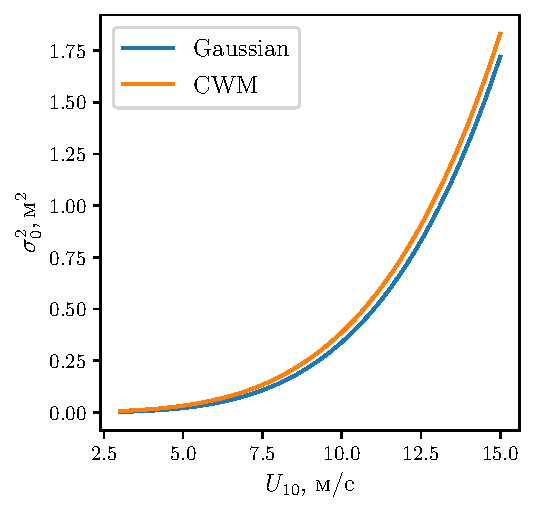
\includegraphics[width=0.6\linewidth]{figs/cwm_variance}
    \caption{}
    \label{fig:}
\end{figure}


\begin{figure}[H]
\centering
\makeatletter
    \@for\i:={1,2}\do{
    \begin{subfigure}{0.45\textwidth}
        \centering
        \includegraphics[width=\linewidth, page=\i]{figs/cwm_demo}
        \subcaption{}
        \label{subfig:cwm_demo\i}
    \end{subfigure}
}

\label{fig:cwm_demo}
\caption{
    Сравнение характеристик заостренной и обычной поверхностей на примере одной
    синусоиды (эффект заострения усилен для наглядности): \\
    \subref{subfig:cwm_demo1} поле высот;
    \subref{subfig:cwm_demo2} поле полных наклонов;
    Синей линией отмечена синусоида, оранжевой -- трохоида.
}
\makeatother
\end{figure}



\begin{figure}[H]
\centering
\makeatletter
    \@for\i:={1,2,3}\do{
    \begin{subfigure}{0.45\textwidth}
        \centering
        \includegraphics[width=\linewidth, page=\i]{figs/cwm_demo_1d}
        \subcaption{}
        \label{subfig:cwm_modeling\i}
    \end{subfigure}
    %\hfill
}

\label{fig:cwm_modeling}
\caption{
    Сравнение основных характеристик реализаций заостренной и обычной
    морских поверхностей: \\
    \subref{subfig:cwm_modeling1} поле высот;
    \subref{subfig:cwm_modeling2} поле наклонов вдоль направления
    распространения волнения;
    \subref{subfig:cwm_modeling3} поле наклонов перпендикулярное направлению
    распространения волнения;
    Синей линией отмечена обычная поверхность, оранжевой -- заостренная.
}
\makeatother
\end{figure}

\begin{figure}
    \centering
    \begin{subfigure}{0.49\linewidth}
        \centering
        \includegraphics[width=1\linewidth]{figs/mirror_dots_Ku.png}
        \caption{}
        \label{subfig:mirror_dots_1}
    \end{subfigure}
    \begin{subfigure}{0.49\linewidth}
        \centering
        \includegraphics[width=1\linewidth]{figs/mirror_dots_Ku.png}
        \caption{}
        \label{subfig:mirror_dots_2}
    \end{subfigure}
    \caption{ Распределение углов отклонения от направления зеркального
    отражения для 
    \subref{subfig:mirror_dots_1} Ku-  и 
    \subref{subfig:mirror_dots_2} Ka- диапазонов}
\end{figure}


\begin{figure}[h]
    \centering
    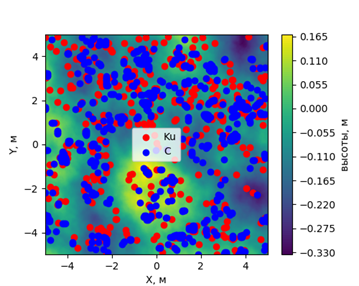
\includegraphics[width=0.6\linewidth]{figs/mirror_dots_distr.png}
    \caption{Распределение зеркальных точек на поверхности высот для Ku- и
    Ka-диапазонов. {\color{red}  перерисовать картинку для нужного диапазона!}}
    \label{fig:}
\end{figure}



%%Здесь начинается не понятный для меня момент. Шулейкин в \cite{shuleykin} при
%выводе орбитальных скоростей пользуется трохоидальной моделью поверхности, т.е.
%фактически орбитальные скорости \eqref{eq:orbital_velocity} были изначально
%получены для заостренной морской поверхности. 

%Не получается ли у нас так, что для обычной (синусоидальной поверхности)
%горизонтальная орбитальных скоростей нет как следствие отсутствия вращения
%частицы, а частица двигается просто со скоростью распространения волны? %должна быть равна всегда скорости
%распространения волны?
%Если мы представим одну синусоиду и будем наблюдать за одной точкой на ней, то
%она будет перемещаться только по вертикальной оси со скоростью
%$\pdv{\zeta}{t}$, а поскольку производная  $\pdv{x}{t} = 0$

%Поэтому мы можем записать орбитальную скорость $v_{\perp}$ в плоскости азимута
%\begin{equation}
    %v_{\perp} = + \fullsum \omega_n(\kappa_{nm}) A_n(\vec \kappa_{nm}) \cos(\fullphase)
%\end{equation}

%Получаем выражения для орбитальных скоростей $v_x$ и $v_y$
 %\begin{equation}
    %\begin{gathered}
        %v_x = \dv[]{x_0}{t} = \cos \phi_0 \fullsum \omega_n(\kappa_{nm}) A_n(\vec
        %\kappa_{nm}) \cos(\fullphase) \\
        %v_y = \dv[]{y_0}{t} = \sin \phi_0 \fullsum \omega_n(\kappa_{nm}) A_n(\vec
        %\kappa_{nm})\cos(\fullphase), \\
    %\end{gathered}
%\end{equation}
%где \where{$\phi_0$}{направление распространения волнения}.

%Для трехмерного случая Пирсон \cite{pierson} представил решение линеаризованных
%уравнений движения для невязкой жидкости в лагранжевых координатах. Он показал,
%что в глубокой воде положение частиц на свободной поверхности задается
%параметрическим уравнением трохоиды


%\begin{equation}
    %\begin{gathered}
        %v_x(\vec r(t), t) = \dv[]{x}{t} = \pdv[]{x}{x_0}\dv{x_0}{t} + \pdv{x}{t} \\

        %%v_y = \dv[]{y}{t} = \pdv[]{y}{y_0}\dv{y_0}{t} + \pdv{y}{t}
    %\end{gathered}
%\end{equation}

%\newpage

%%\bibliography{main}
\newpage
\section*{Заключение}

\bibliographystyle{IEEEbib}
\bibliography{main}
%%\printnomenclature[5em]
\end{document}

